\begin{figure}
	\centering
	\begin{minipage}[t]{.5\textwidth}
		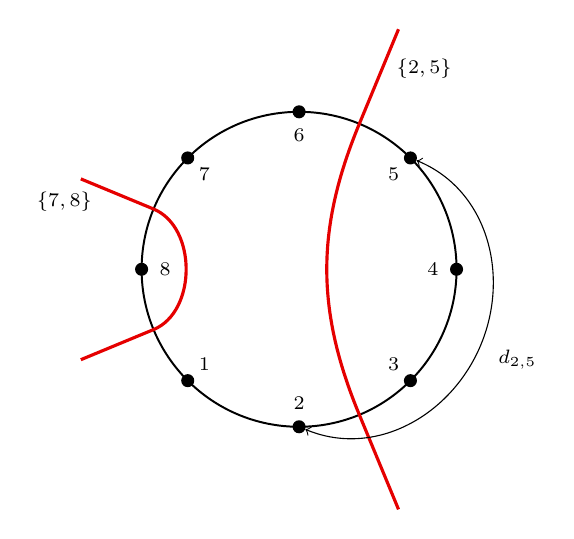
\begin{tikzpicture}[font=\scriptsize, node/.style={circle,thick,draw},
		l_2/.style={line width =0.25mm},
		scale=1, transform shape]
			% equidistant points and arc
			\foreach \x [count=\p] in {0,...,7} {
				\node[shape=circle,fill=black, scale=0.5] (\p) at (\x*45-135:2) {};
			};
			\foreach \x [count=\p] in {0,...,7} {
				\draw (225 + \x*45:1.7) node {\p};
%				\draw (-30-\x*60:2.4) node {$\bar{\p}$};
			}; 
			\draw[l_2] (4) arc (0:360:2);
			
			\draw[line width=0.4mm, red!90!black] (67.5:3.3) to [out=-112.5,in=67.5] (67.5:2) to [out=-112.5,in=112.5] (-67.5:2) to [out=-67.5, in=112.5](-67.5:3.3);
			\node (cut1) at (58:3) {$\{2, 5\}$};
			
			\draw[line width=0.4mm, red!90!black] (157.5:3) to [out=-22.5,in=157.5] (157.5:2) to [out=-22.5,in=22.5] (-157.5:2) to [out=-157.5, in=22.5](-157.5:3);
			\node (cut2) at (164:3.1) {$\{7, 8\}$};
			
			\node (a) at (-22.5:3) {$d_{2, 5}$};
			\draw[<->] (2)  to [out=-22.5,in=-112.5] (-22.5:2.5) to [out=67.5,in=-22.5](5);
%			\node (b) at (-67.5:2.8) {$d_{1, 4}$};
%			\draw[<->] (1)  to [out=-67.5,in=-157.5] (-67.5:2.5) to [out=22.5,in=-67.5] (4);
			
			\node (bottom) at (0, -2.8) {};
			%		\draw[dashed] (1) -- (3) -- (5) -- (1);
			% axes
			%		\draw [dotted, gray] (-2.6,0) -- (2.6,0);
			%		\draw [dotted, gray] (0,-2.15) -- (0,2.15);
		\end{tikzpicture}
	\end{minipage}
	\caption{Examples of cuts (red).
	We imagine a cut as a chord connecting the midpoints of its edges.
	The demand $d_{2, 5}$ crosses the cut $\{2, 5\}$ and is parallel to the cut $\{7, 8\}$.
	The cuts $\{2, 5\}$ and $\{7, 8\}$ are parallel.}
	\label{fig:cut-example}
\end{figure}